\subsection{Precursor chemistry}

A detailed discussion of the time histories of measured species was presented in our previous work~\citep{clark2025}. The performance analysis of six kinetic mechanisms indicated that FFCM2~\citep{ZDV2023} provides the best agreement across the entire temperature range, especially for $\mathrm{CH_4}$ conversion and $\mathrm{C_2H_2}$ yield, but it does not include PAH chemistry necessary for inception and surface growth, so it cannot be used for soot modeling. As shown in Fig.~\ref{fig:CH4_C2H2_A2_A2R5_CRECK}a and b, the CRECK mechanism predicts $\mathrm{CH_4}$ and $\mathrm{C_2H_2}$ mole fractions in close agreement with the measurements, considering their uncertainty range. CRECK includes the PAH chemistry necessary for soot inception and surface growth. Fig.~\ref{fig:CH4_C2H2_A2_A2R5_CRECK}c and d depict the mole fractions of A2 and A2R5, which similarly increase with time. For T$_5$$>$2200~K, the mole fraction of PAHs reaches its peak and gradually decreases within 1~ms, primarily due to conversion to C$_2$H$_2$ rather than soot inception. The mole fraction of A2 and A2R5 sampled at 1~ms follows the well-known bell-shaped behavior with the peak near 2200~K. The analysis of the carbon mass fraction (CMF) of precursors over the studied T$_5$ range indicated that A2 and A2R5 are the major contributors to soot inception due to their larger CMFs compared to the other precursors. The initial composition of soot is dictated by the H/C ratio of constituent precursors, which changes within a narrow range, slightly decreasing from 0.8 at 1875~K to 0.67 at 2355~K.


\begin{figure}[!t]
	\centering
	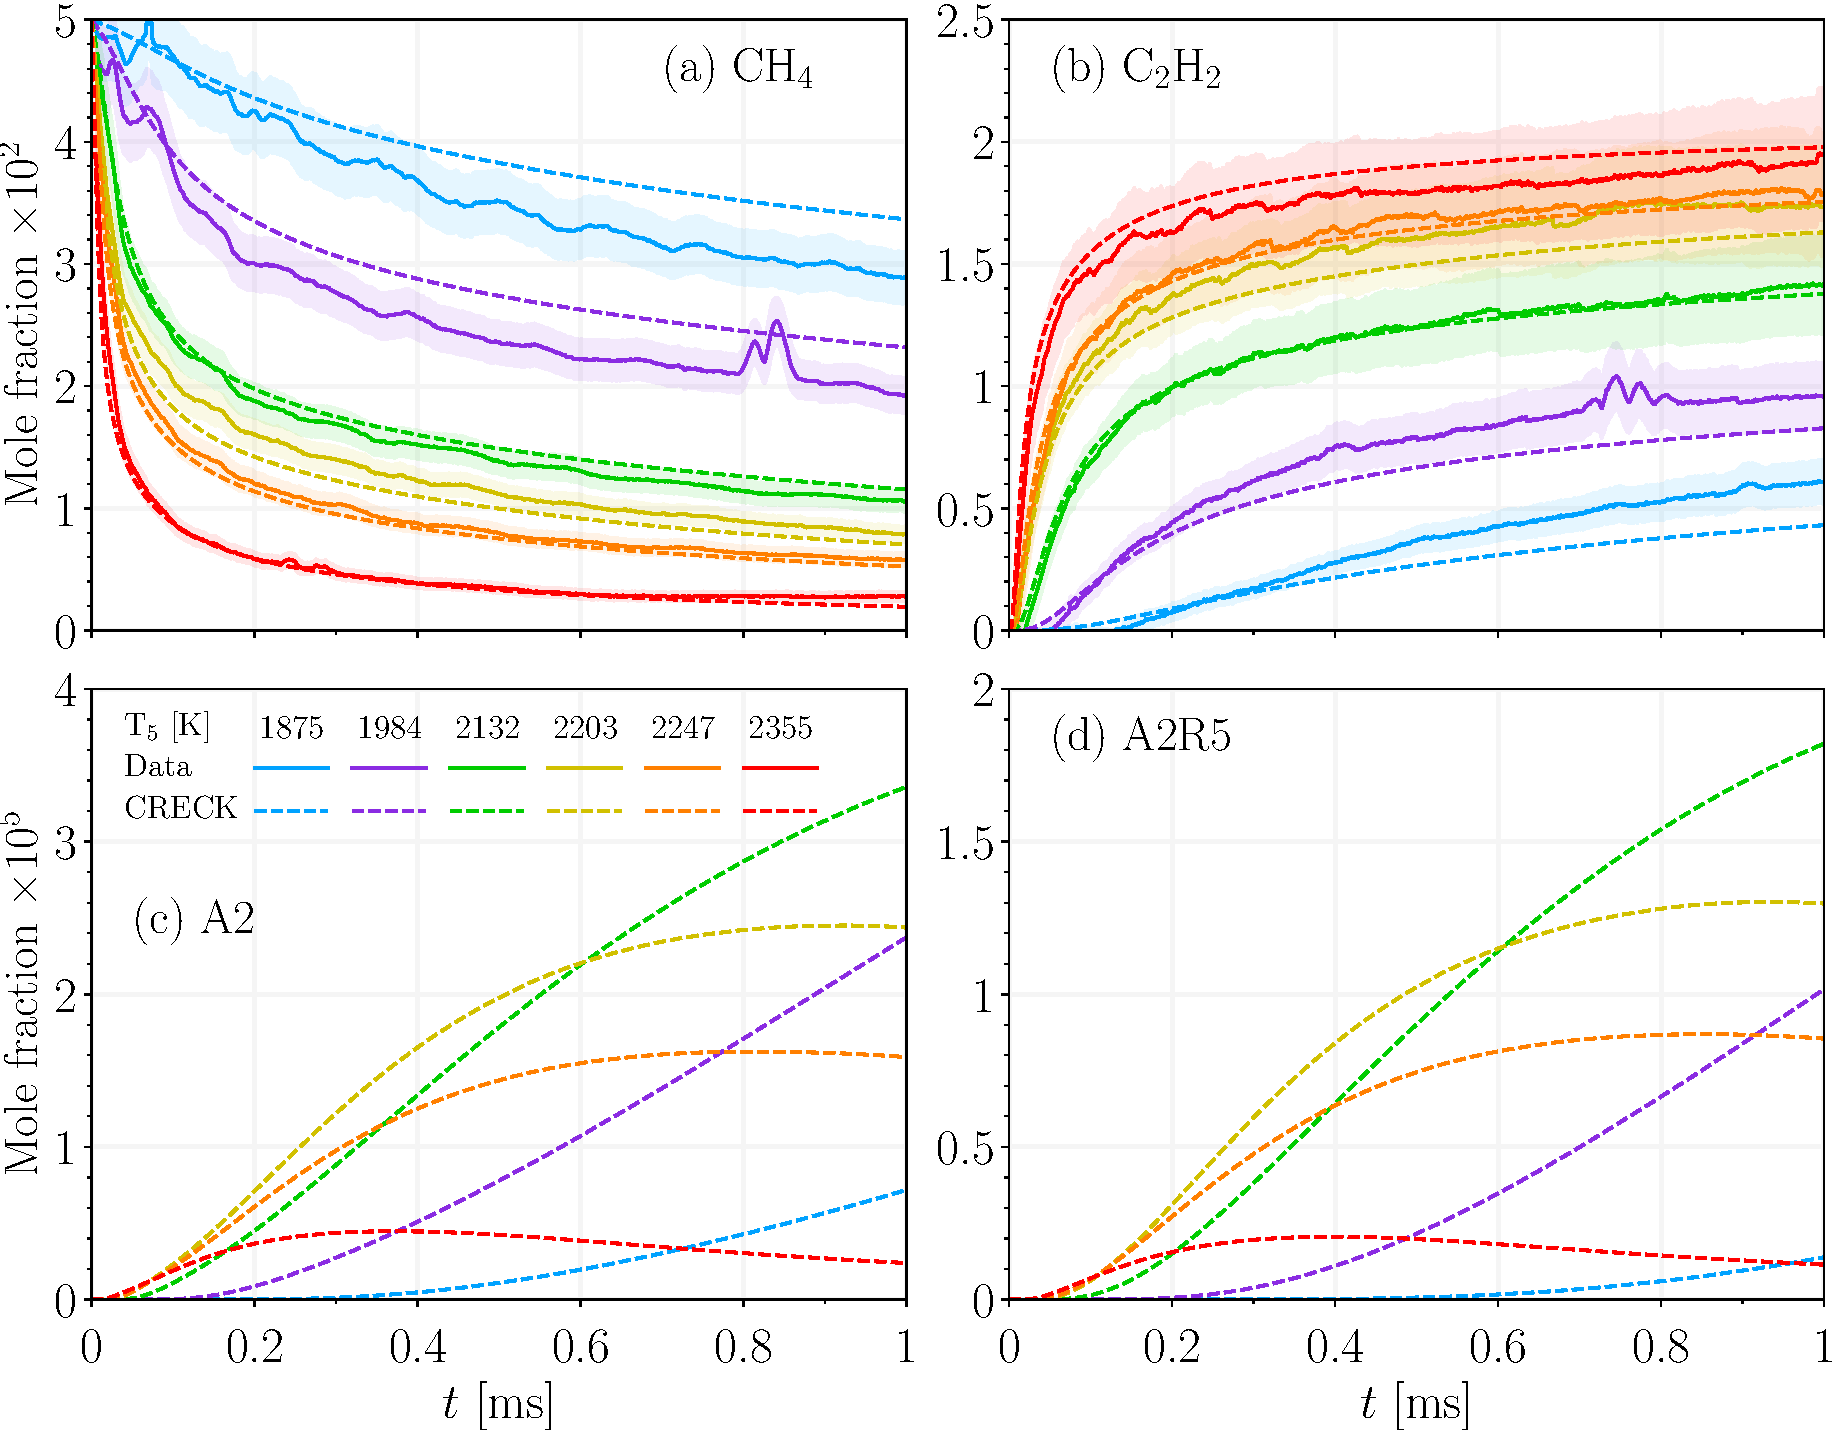
\includegraphics[width=0.95\textwidth]{Figures/Results/Paper3/CH4_C2H2_A2_A2R5_CRECK.pdf}
	\caption{The time history of (a) CH$_4$ and (b) C$_2$H$_2$ predicted using CRECK mechanisms in close agreement with the laser absorption measurements. The shaded area represents the uncertainty in the measurements.}
	\label{fig:CH4_C2H2_A2_A2R5_CRECK} 
\end{figure}






